\documentclass[12pt]{article}
\usepackage{amsmath}
\usepackage{amsfonts}
\usepackage{amssymb}
\usepackage{graphicx}
\usepackage[left=2cm,right=2cm,top=2cm,bottom=2cm]{geometry}

\usepackage[pdftex]{color}
\usepackage{multicol}
\newcommand{\cred}{\textcolor{red}}
\newcommand{\cblue}{\textcolor{blue}}
\newcommand{\cgreen}{\textcolor{green}} 

\usepackage{listings}
\definecolor{codegreen}{rgb}{0,0.6,0}
\definecolor{codegray}{rgb}{0.5,0.5,0.5}
\definecolor{codepurple}{rgb}{0.58,0,0.82}
\definecolor{backcolour}{rgb}{0.95,0.95,0.92}
\lstdefinestyle{mystyle}{
	backgroundcolor=\color{backcolour},   
	commentstyle=\color{codegreen},
	keywordstyle=\color{magenta},
	numberstyle=\tiny\color{codegray},
	stringstyle=\color{codepurple},
	basicstyle=\footnotesize,
	breakatwhitespace=false,         
	breaklines=true,                 
	captionpos=b,                    
	keepspaces=true,                 
	numbers=left,                    
	numbersep=5pt,                  
	showspaces=false,                
	showstringspaces=false,
	showtabs=false,                  
	tabsize=2
}
\lstset{style=mystyle}

\begin{document}

\hfill \today

\begin{center}
\textbf{\Large  Learn \LaTeX\  by Examples}
\end{center}

\noindent \hrulefill

\noindent \textbf{1. Examples of lists}\\
 
\textit{Unnumbered list.}
\begin{itemize}
\item First item is nothing!
\item Second item is unknown.
\end{itemize}

\vspace{0.25in}

\textit{Numbered list.} 
\begin{enumerate}
\item $\alpha, \beta$, $\alpha$, $\omega$, $\Omega$
\item $f(x)=\dfrac{x^2+4}{x+2}$.
\item Temperature is $75^\circ$ F.
\end{enumerate}

\vspace{0.25in}

\textit{Other styles.}  
\begin{enumerate}
\item[a.] 
\item[b.] 
\end{enumerate}

\begin{itemize}
\item[i.] 
\item[ii.] 
\end{itemize}


\newpage
\noindent \textbf{2. Examples of mathematical expressions} 


$x=2$

\[ x=2\] 

\begin{equation}\label{eq1}
x^2-4=0
\end{equation}

From equation (\ref{eq1}), we get $x=\pm 2$.
%
\[\sin2\theta = 2\sin\theta\cos\theta, \quad \cos2\theta = 2\cos^2\theta -1 =1 -2\sin^2\theta\]
%
$$f(x)=\int_0^x g(t)\, dt \implies f'(x) = g(x)$$

Roots of a quadratic equation $ax^2+bx+c=0$ is given by 
\begin{equation}
x_{1,2}=\frac{-b\pm \sqrt{b^2-4ac}}{2a}
\end{equation} 

\begin{equation*}
\int_0^1 \frac{4}{1+x^2}\, dx = \pi
\end{equation*} 



\begin{eqnarray*}
x_{n+1} &= & x_n-\frac{f(x_n)}{f'(x_n)}\\
x_{n+1} &=& x_n-2\frac{f(x_n)}{f'(x_n)}\\
x_{n+1} &=& x_n-\frac{f(x_n)}{\sqrt{[f'(x_n)]^2-f(x_n)f''(x_n)}}
\end{eqnarray*}

\newpage
\noindent \textbf{3. Examples to create a table} 

\begin{center}
\begin{tabular}{|c|c|c|c|c|c|}
\hline
Food  &  protein & carbohydrate & fat & salt & calcium\\
\hline
	 A	&   0    &     15 	&     
	   10 		&    10 &    15\\
	 B	&  30    &    20   	&     	20   & 10   &  20\\
	 C	&  20    &    25    &    	10   & 20  &   15\\
	 D	&  30    &   15     &  		30    & 10 &    20\\
	 E	&  10    &  15       & 		0    & 20 &     5\\
\hline
\end{tabular}
\end{center}
\vspace{0.1in}

Table in math environment (array). 
\[
\begin{array}{|c|c|c|}
\hline
n & t & y(t)\\
\hline
0 & 0.00 & 0.5000\\
1 & 0.25 & 0.5615\\
2 & 0.50 & 0.6204\\
3 & 0.75 & 0.6752\\
4 & 1.00 & 0.7251\\
\hline
\end{array}
\]

Math expressions with matrix and vectors:
\[
A=
\left[
\begin{array}{rrr}
3&0&1\\
0&3&1\\
1&1&3
\end{array}
\right]
,\quad
A^{-1}= \frac{1}{21}\left[\begin{array}{rrr}
8 & 1 & -3 \\
1 & 8 & -3\\
-3 & -3 & 9
\end{array}\right], \quad
{\bf x}=
\left[
\begin{array}{r}
x_1\\
x_2\\
x_3
\end{array}
\right], \quad
{\bf b}=
\left[
\begin{array}{r}
4\\
4\\
5
\end{array}
\right]
\]

\newpage
\noindent \textbf{4. Example on how to insert a figure in the text}
%%%%%%%%%%%%%%%%%%%%%%%%%%%%%%%%%%%%%%%%%%%%
\begin{figure}[htb]
\begin{center}
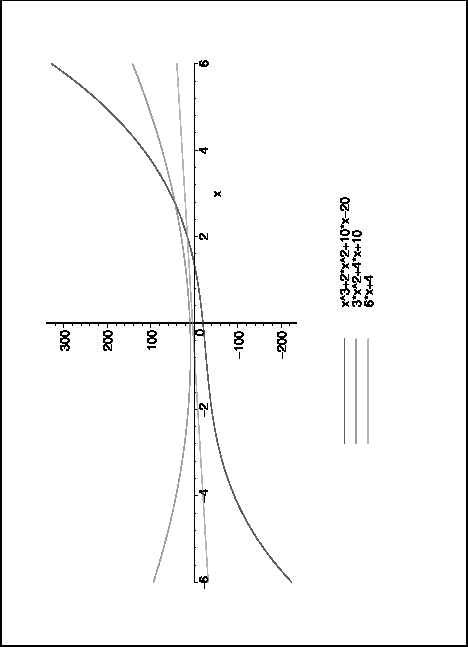
\includegraphics[width=2.in]{plot1.jpg} 
\caption{Put caption of the figure here}
\end{center}
\end{figure}

\begin{figure}[htb]
\begin{center}
\rotatebox{270}{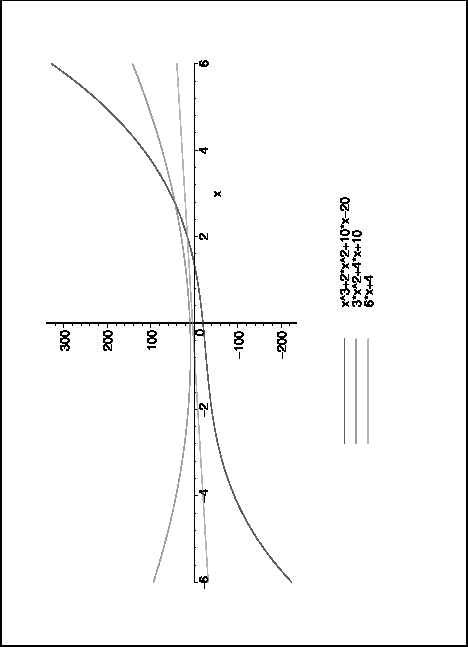
\includegraphics[width=3.15in]{plot1.jpg}}
\end{center}
\caption{Rotated the figure by 270$^\circ$, resized and placed at the center.}
\end{figure}

\newpage
\noindent \textbf{5. Here is an example of \texttt{verbatim}.} 

\begin{verbatim}
Median age at First Marriage, 1890-2010
Source: U.S. Bureau of the Census, www.census.gov
Year     Men      Women
1890     26.1     22.0
1900     25.9     21.9
1910     25.1     21.6
1920     24.6     21.2
1930     24.3     21.3
1940     24.3     21.5
1950     22.8     20.3
1960     22.8     20.3
1970     23.2     20.8
1980     24.7     22.0
1990     26.1     23.9
2000     26.8     25.1
2010     28.2     26.1
\end{verbatim}

\noindent \textbf{6. Here is an example of \texttt{lstlisting}.} 
\begin{lstlisting}[language=Python]
#!/usr/bin/env python3 
import numpy as np
"""
Purpose: To create a magic square of NxN matrix with NumPy (N must be odd)

"""

def gen_magic_square(N):
    magic_square=np.zeros((N,N),dtype=int)
    n=1
    i, j = 0, N//2
    while n <= N**2:
        magic_square[i,j] = n
        n += 1
       newi, newj = (i-1) % N, (j+1) % N
       if magic_square[newi, newj]:
           i += 1
       else:
           i, j = newi, newj
    return magic_square

if __name__== '__main__':
    A=gen_magic_square(3)
    B=gen_magic_square(5)
    C=gen_magic_square(7)
    print(A); print(B); print(C)
\end{lstlisting}

\end{document}

